\documentclass[tikz,border=2pt]{standalone}
\usepackage{amsmath}
\usepackage{pgfplots}
\pgfplotsset{compat=1.18}
\usetikzlibrary{arrows.meta}

\begin{document}
% In one variable: f(x)=2x is linear (a line through the origin, f(0)=0); g(x)=2x+1 is affine
% (the same line shifted by b=1), so g(0)≠0 and g(x+y)≠g(x)+g(y).
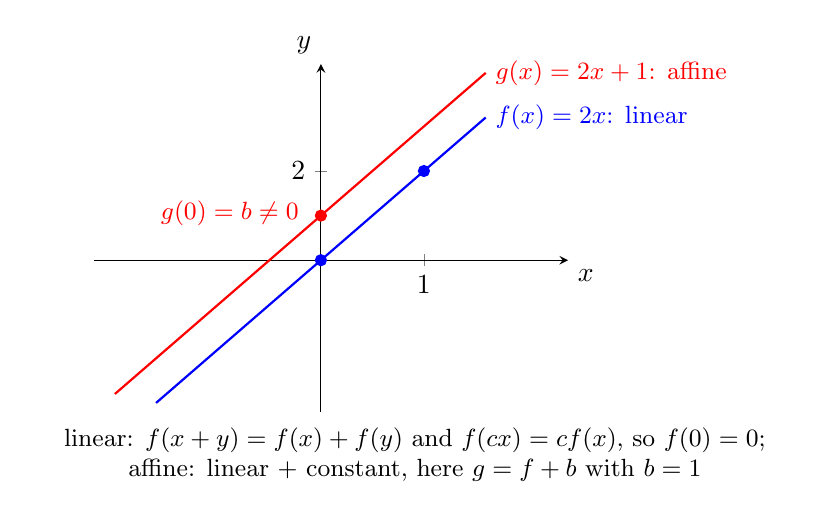
\begin{tikzpicture}
	\begin{axis}[
		axis lines=middle,
		xmin=-2.2, xmax=2.4,
		ymin=-3.4, ymax=4.4,
		xtick={1}, ytick={2},
		xlabel={$x$}, ylabel={$y$},
		xlabel style={below right}, ylabel style={above left},
		samples=2, clip=false,
		width=7.6cm, height=6cm
		]
		\addplot[thick, blue, domain=-1.6:1.6] {2*x};
		\addplot[thick, red, domain=-2:1.6] {2*x+1};
		\addplot[only marks, mark=*, blue] coordinates {(0,0) (1,2)};
		\addplot[only marks, mark=*, red] coordinates {(0,1)};

		\node[blue, anchor=west, font=\small] at (axis cs:1.6,3.2) {$f(x)=2x$: linear};
		\node[red, anchor=west, font=\small] at (axis cs:1.6,4.2) {$g(x)=2x+1$: affine};
		\node[red, anchor=east, font=\small] at (axis cs:-0.12,1.05) {$g(0)=b\neq0$};
	\end{axis}
	\node[anchor=north, font=\small, align=flush center, text width=9.6cm] at ([yshift=-2pt]current axis.outer south) {linear: $f(x+y)=f(x)+f(y)$ and $f(cx)=cf(x)$, so $f(0)=0$; affine: linear $+$ constant, here $g=f+b$ with $b=1$};
\end{tikzpicture}
\end{document}
